% !TEX root = ../TUCthesis.tex

%************************************************
\chapter{Implementation of Heterogeneous WSN}\label{ch:Implementation}
%************************************************

The \acp{SN} in the heterogeneity network model are not centrally operated to avoid single point of failure. Therefore they act independently to co-ordinate and communicate with their neighbors to resolve contentions among the \acp{SN} for heterogeneity layer access. This approach requires frequent message exchanges among the nodes. Therefore, we need an efficient routing methodology to minimise the beacon exchange count and further initiate the data transfer via heterogeneity in a contention free slot. 

In order to realise the benefits of deploying heterogeneity in a network, we simulate heterogeneity along with \ac{CTP} algorithm. This chapter describes the simulation methodology and programming structure of heterogeneity concept. In the first section, Platforms used \ref{sec:PlatformsUsed}, we describe the hardware and software components used for simulating the network model. In the second section, Design Components \ref{sec:DesignComponents}, we provide an overall picture of heterogeneity model and further describe the TinyOS components and interfaces involved in the design phase. This also explains the importance of \acp{CTP} module for our routing model. In the third section, Control Plane Design \ref{sec:ControlPlaneDesign}, a detailed analysis of the routing mechanism in heterogeneity is provided. It describes three aspects of heterogeneity: 1. how the protocol finds the route to destination heterogeneous node 2. the criterion to decide one of the possible routes found by route discovery phase 3. how the final selected route is represented in the heterogeneity model. As a follow up to the routing model, the subsection, Routing Implementation, conforms the routing model requirements with heterogeneity model. This subsection also contains the packet contents of message exchanges in heterogeneity. The packets in our network model serve as an important aspect to realise information exchange among \acp{SN}. In the fourth section, Heterogeneity Specific Implementations \ref{sec:heterogeneitySpecificImplementations}, we provide a detailed explanation of data structures involved in running the heterogeneity model. The explanation focuses on two major aspects: 1. how these data structures are linked to each other and 2. how their interdependency act as an important tool to regulate state change in heterogeneity. In the fifth section, Data Plane Design \ref{sec:DataPlaneDesign}, data transmission in one hop and two hop neighborhood through heterogeneity is explained. In the final section \ref{sec:processModel}, we present the flow diagrams to sketch the life cycle of heterogeneity model. 

%************************************************
\section{Platforms Used} \label{sec:PlatformsUsed}
%************************************************

This section is divided in two parts: hardware components and software components.

    %************************************************
    \subsection{Hardware Components}
    %************************************************
    
    The hardware used for implementation are Telosb motes \cite{datasheet:Telosb}. This sensor platform was originally developed by the University of California, Berkeley by TinyOS developers. It features the 8MHz Texas Instrument MSP430 (the MSP430F1611) microcontroller with a 10 kBytes internal RAM and a 48 kBytes program Flash memory, IEEE 802.15.4 CC2420 radio chip, data transfer rate up to 250kbps, integrated onboard antenna, 1MB external flash for data logging, programming and data collection via USB, sensor suite including integrated light,  temperature and humidity sensor and runs on TinyOS 1.1.10 or higher.
    
    %************************************************
    \subsection*{MSP430 Microcontroller}
    %************************************************
    
    The MSP430 \cite{website-MSP430} is a low-cost microcontroller generally used for low powered embedded devices. It has a 16-bit \ac{RISC} CPU with an instruction cycle time of 125$nS$. The device is highly optimised for low energy consumption and high code efficiency. It supports six different low-power modes to disable unnecessary running of clocks and CPU. It is capable of wake-up times below 1$\\muS$, which allows the microcontroller to stay in low power mode for longer period of time and thus maximising the available energy budget. The power consumption in active mode is about 330$\mu A$ at 1MHz with 2.2V. In idle mode the microcontroller needs less than 1$\mu A$. The supply voltage should be in the range of 1.8V to 3.6V.
    
    %************************************************
    \subsection*{CC2420 Radio}
    %************************************************
    
    It is a 2.4GHz IEEE 802.15.4 complaint RF transceiver  \cite{TI:cc2420}. It is specially designed for low power embedded devices. Some of the important features include: extensive hardware support for packet handling, data buffering, burst transmissions, data encryption, data authentication, clear channel assessment, link quality indication and packet timing information.
    
    %************************************************
    \subsection{Software Components}
    %************************************************
    
    We have compiled our heterogeneity code in TinyOS which uses nesC programming language. In addition to this, we have also used COOJA simulator \cite{cooja:Contiki} to simulate the compiled code in a virtual \ac{WSN} environment. Cooja is a java based simulator for emulating \acp{SN} of certain platforms at hardware level. This allows faster and precise inspection of the model behaviour for the compiled TinyOS code.

%**********************************************************
\section{Design Components} \label{sec:DesignComponents}
%**********************************************************
In the first subsection, we will discuss heterogeneity implementation possibilities with a focus on energy and computational power. In the second part, we will briefly explain about the working of heterogeneity layer and in the final subsection, we will talk about the general TinyOS components required for implementing heterogeneity.

    %************************************************
    \subsection{Heterogeneity Possibilities}
    %************************************************
    
    From the literature survey in chapter \ref{ch:literature}, we have explored several possible dimensions of  heterogeneity implementation including increased energy, computational power, memory, wireless range, etc. for a particular group of \acp{SN}. With \acp{CTP} being the most widely used protocol, we implement it as the baseline for collecting data generated at a \acp{SN} and for the sake of simplicity, we rely on the parameters energy and computational complexity throughout the remainder of the report. Also, we depend on these parameters to perform a comparative analysis of heterogeneity with \acp{CTP}.
    
    %************************************************
    \subsection{Outline}
    %************************************************
    
    The heterogeneity set up requires \ac{CTP} implementation (provided in \cite{tinyOS:ctpImplementation}) at back end. \ac{CTP} is responsible for building and maintaining minimum cost trees to nodes which advertise themselves as roots based on \ac{ETX} parameter. Messages are sent and received via \ac{CTP} send and receive interfaces. On top of the \ac{CTP} layer, we implement the heterogeneity layer. The tasks performed by this layer are sequential and event-driven. \acp{SN} respond to different events and thus change their states on subsequent events reception or triggering. We will discuss more about states and flow diagrams in section \ref{sec:processModel}. These states are stored as global variables  or well-defined structs in the implementation. In summary, the \acp{WSN} operates in an endless loop in the following order:
    
    \begin{enumerate}
        \item Beacon based \ac{PC} announcement in one and two hop neighborhood: Each \ac{PC} participates in the periodic advertisement of their computational power availability to their one and two hop neighbors.
            
        \item Selective \ac{RTS} response by \ac{SN} to the beacon announcement: The notion of \ac{RTS} concept used in heterogeneity layer is equivalent to sending a request packet to check the \ac{PC} availability before the actual transmission of data. The packet requests a unique time slot for the intended sender and thus resolves the conflict of multiple data senders to one \ac{PC}.
        
        \item \ac{CTS} response by \ac{PC}: Based on the earliest \ac{RTS} request, a \ac{CTS} response is generated by the \ac{PC} for the intended sender. The notion of \ac{CTS} response implies that the \ac{PC} will have to send a clear to send signal before the intended \ac{SN} can initiate the data transmission. Until the intended sender gets a \ac{CTS} response, it participates in \ac{CTP} collection for sending it's data.
        
        \item Data transfer via heterogeneity layer: On reception of \ac{CTS} response by the intended sender, the data transmission phase starts for the time period the intended sender requests. 
        
        \item Data collection via \ac{CTP} from \ac{PC} to \ac{BS}: On completion of data sending by a \ac{SN} to \ac{PC}, the final computed data is added to the data collection queue and thus it reaches the \ac{BS} via \ac{CTP}.
    \end{enumerate}
    
    We will have a closer look at the detailed implementation of the heterogeneity set up in the coming sections and subsections. 
    
    %************************************************
    \subsection{TinyOS Components}{\label{subsec:tinyOSComponents}}
    %************************************************
    
    In this subsection, we will discuss about the interfaces and wiring required for implementing heterogeneity.
    
    \begin{enumerate}
        \item General Interfaces: Following are the commonly used interfaces required for the implementation: 
    
            \begin{itemize}
                \item Boot: It is required to boot a \ac{SN}. the boot interface signals Boot.booted() event on successful booting of the device.
                
                \item SplitControl: It is used to start and stop services of the radio transceiver. It is wired to ActiveMessageC component.
                
                \item StdControl: This interface is provided by Collection protocol. StdControl interface  controls the state of \ac{CTP} routing by setting/resetting the routing state once the routing layer of \ac{CTP} starts or stops respectively.
                
                \item Leds: This is used for controlling the led lights on the Telosb. We use light patterns to indicate transmissions and receptions in our application. The interface is wired to ledsC component and provides methods such as LedsToggle, LedsOn or LedsOff for the leds.
            \end{itemize}
        
        \item CTP-based Interfaces: These interfaces are provided by \ac{CTP} to send and receive messages via the collection tree. 
        
            \begin{itemize}
                \item RootControl: This interface is used to advertise a particular \ac{SN} as a root node of the \ac{CTP} tree.
            
                \item {\label{item:Send}} Send: It is used to send messages via \ac{CTP} protocol through the collection tree. This interface is wired to CollectionSenderC component provided by \ac{CTP}.
                
                \item Receive: It is used to receive messages sent via Send interface in \ref{item:Send}. The messages received via this interface are exclusively sent via \ac{CTP} protocol. Messages sent via other sending interfaces, which are not wired to CollectionSenderC, do not get routed via \ac{CTP}. This distinction helps in implementing an abstraction layer over \ac{CTP} on which we will build our heterogeneity model and thus keep our data exchange model separate from \ac{CTP} communications.
                
                \item CtpInfo: This interface provides methods to obtain \ac{ETX} information about the current \ac{SN}. It is also wired to CollectionC component of \ac{CTP} so that we could obtain the \ac{ETX} metric used in setting up the collection tree. This metric is also updated periodically by \ac{CTP} and therefore keeps the heterogeneity model remians up to date with changes in \ac{ETX} metric.
                
                \item Timer: This timer is fired to perform routing via \ac{CTP}. Only when this timer is fired, the \ac{SN} announces itself as a part of \ac{CTP} and further acknowledges itself as a member of \ac{CTP} tree. 
            \end{itemize}
    \end{enumerate}
        
%************************************************
\section{Control Plane Design } \label{sec:ControlPlaneDesign}
%************************************************
    
This section describes the advertisement phase of a \ac{PC} and \ac{PC} selection phase of an intended sender. We will first describe the routing model and then explain the routing implementation phase of our design.

    %************************************************
    \subsection{Routing Model}
    %************************************************
    
    In this subsection, we will look at the route discovery, route selection, route representation and data forwarding phases of heterogeneity.
    
    \begin{enumerate}
        \item Route Discovery: To derive the route discovery mechanism implemented in our design, we will continue from the previous description on route discovery in section \ref{enumerate:RouteDiscovery} (in chapter \ref{ch:Background}). 
        
        \par
        In our heterogeneity model, we perform the route discovery phase by maintaining an array of known \acp{PC} in at most two hop neighborhood. Therefore, We can say that the route discovery is done proactively because we know exact route from sender to \ac{PC} in advance. A sorting algorithm periodically sorts this array for the optimal selection of \ac{PC} at constant run time ($O(1)$) (explained in detail in sections  \ref{item:routeSelection} and \ref{sec:heterogeneitySpecificImplementations}). Further, to ensure collision free data transmission, a \ac{RTS} packet is sent to the first member of the \ac{PC} array to verify if the recipient is free. 
        
        \par
        The \ac{PC} reply packet carries routing information to stimulate data transmission by sender. We can utilize the concept of message pools to avoid the \ac{PC} route reply packet transmission. The concept of message pool can be exploited in two ways: either we maintain separate queue for each of the possible senders or accept data from all possible senders in one queue at any point of time. Although these methods solve the problem of sender fairness, yet these pools can be memory intensive in high traffic scenario. Also, to implement the latter scenario, we will first have to sort similar data in the message pool and then process them in ordered way. One more drawback of pooling approach is frequent back-offs while sending stream of data because multiple nodes will try to to get channel access while sending to one \ac{PC} and hence would not get clear channel assessment very often. This can finally lead to low data delivery ratio. Therefore, instead of this pooling approach, we have chosen to reserve the processing center for a particular \ac{SN} and only after the reservation confirmation, the intended sender can send their data for processing. We also assume here that each of the \ac{SN} can send only one type of data for the allotted reservation period. A \ac{PC} confirms its own reservation via \ac{RREP} packet to the sender on first come first serve basis. It waits for a certain amount of time to receive data. In case of no reception after passage of allotted time period, it again starts flagging itself as an available \ac{PC} to the \acp{SN} in one or two hop neighborhood. 

        \item \label{item:routeSelection} Route Selection: In the previous discussion on route selection in \ref{enumerate:RouteSelection} (in chapter \ref{ch:Background}), we have explained the possible ways of route selection. Now, we will discuss how we achieve this in our heterogeneity design.
        
        \par
        We use \ac{CTP} to get \ac{ETX} information of the \ac{SN} in order to select the best \ac{PC} for data transmission. As claimed by the authors, \ac{CTP} maintains an updated \ac{ETX} estimate of \acp{SN} on periodic basis. We use these updated \ac{ETX} values for \ac{PC} selection. To extract the \ac{ETX} values, the interface 'CtpInfo.nc' is wired to CTPRoutingEngineP component, which is also provided in the TinyOS \ac{CTP} implementation. This interface provides following useful methods for neighborhood discovery and route selection:
        
        \begin{enumerate}
        	\item getParent() -> Gets the parent of the node in the tree.
        	
        	\item getEtx() -> Gets the \ac{ETX} for the current path to the root through the current parent.
        	
        	\item triggerRouteUpdate() -> Informs the routing engine that sending a beacon soon is advisable.
        	
        	\item numNeighbors() -> Gets number of neighbours.
        	
        	\item getNeighborLinkQuality() - Gets the Link Quality of a neighbor. 
        	
        	\item getNeighborAddr() -> Gets the address of the neighbor.
        \end{enumerate}
        
        \par
         For the route selection process, we propagate the \ac{ETX} information, obtained by  \textbf{getEtx} method, during the beacon broadcasting phase. This value is then used through out in our design and is the building block of optimal \ac{PC} selection. We therefore believe that re-using and keeping an updated copy of this information in the network enhances the network reliability.
        
        \par    
        We have also added an extra method in CTPInfo interface to acquire addresses of all the \acp{SN} in one hop neighborhood. This was done with the help of \textbf{getNeighborAddr} method. This method returns the address of all the \acp{SN} from it's routing table. As mentioned in previous section on route discovery, each \ac{SN} in \ac{CTP} maintains a routing table of size number of neighbors containing neighbor address and other relevant fields. We therefore exploit this routing table information by iterating through all the routing tables for the number of neighbors in one hop neighborhood (provided by CtpInfo numNeighbors method). Further, we store all the neighbor addresses in an array and return it. Although this method is currently not used in the model, but it can be quite useful in improving the network reliability and efficiency by precisely determining the \ac{SN} density around each of the \acp{SN} and further placing a \ac{PC} around it.   
        
        \item Route Representation: We have implemented the idea of route guidance in search phase. However, to make it more efficient, we have blended in the idea of source routing in data transmission phase. This approach will inform the sender about the exact route to destination through which the data transmission phase should take place. In this way we will not waste energy in re-computing the route to destination every now and then. There is also an added benefit to this approach: we do not need to maintain long routing tables as we need only the routing information from the \ac{SN} to the \ac{PC} in one or two hop neighborhood. We therefore do not add routing information for \acp{PC} located at a distance more than two hop and hence avoid maintaining long routing tables and thus leave off the distant \acp{PC}.
        
        \item Auxiliary Components: Apart from the above three routing components, we have also looked into the following aspects: 
    
        \begin{enumerate}
        	\item Route Maintenance
        	\item Route Refreshing
        	\item Route Failure Handling
        	\item Route Invalidation
        	\item Restricted Flooding
        	\item Data Aggregation
        \end{enumerate}
        
        The first four auxiliary components have already been taken care of by re-using the information from \ac{CTP} protocol because the protocol sends beacons every 5ms to update stale route information, if any, in the \ac{WSN}. Also, we have restricted flooding to two hop neighborhood in the route discovery phase. In other phases, we perform unicast transmissions. Moreover, the concept of heterogeneity relies on the notion of data aggregation technique as we send only same type of data to the processing center. This reduces the number of packets flowing through the network which in turn would reduce the overall energy budget of the \acp{SN}.
    
        
    \end{enumerate}
    
    
    %************************************************
    \subsection{Routing Implementation}
    %************************************************
    
    The routing implementation is summarised in following points: 
    
    \begin{enumerate}
        \item As discussed before, route discovery phase begins with beacon advertisement of \acp{PC}. Each node maintains a local copy of the advertising \acp{PC} and use it for route computation phase. Table \ref{tab:Beacon_advertisement} shows the packet contents of beacon advertisement message. 
        
        \begin{table}[h]
    	\caption{Beacon Advertisement} % title name of the table
    	\centering
    	\begin{adjustbox}{max width=\textwidth}
    	
        	\begin{tabular}{|c|c|c|c|} 
        		\midrule
        		Field names: & \ac{PC} ID & \ac{PC} \ac{ETX} &Relayer \ac{ETX} \\
        	    
        	    TinyOS Data Type: & nx\_uint8\_t & nx\_uint16\_t & nx\_uint16\_t \\
        	    
        	    Size(In bytes): & 8 & 16 & 16 \\
        			
        		\hline
        		\end{tabular}
    	\end{adjustbox} 	
    	\label{tab:Beacon_advertisement}
        \end{table}
    
        \item In the next step, a route is selected based on \ac{ETX} values propagated during beacon advertisement.
        
        \item Based on \ac{PC} availability at different moments, we can expect \ac{PC} availability issues. Therefore, we can not rely on static routing table and rather need to determine if the processing centre is available before data transmission. If no \ac{PC} is found free, the data transmission takes place via \ac{CTP}. For determining the availability, the sender sends a \ac{RREQ} to \ac{PC} and in response the \ac{PC} makes a \ac{RREP} to the sender if it finds itself free. Table \ref{tab:CTS_Packet} and shows the contents of \ac{RTS} and \ac{CTS} packets respectively.
        
        \begin{table}[h]
    	\caption{RTS Request Packet} % title name of the table
    	\centering
    	
    	\begin{adjustbox}{max width=\textwidth}
    	\begin{tabular}{|c c c c c|} 
    	
    		\midrule
    		Field names: & Duration & Sender Address & Relayer Address & \ac{PC} Address \\
    		
    	    TinyOS Data Type: & nx\_uint8\_t & nx\_uint8\_t & nx\_uint8\_t & nx\_uint8\_t \\
    		    
    	    Size(In bytes): & 8 & 8 & 8 & 8\\
    			
		\hline
		\end{tabular}
    	\end{adjustbox}
    	\label{tab:RTS_Request_Packet}
        \end{table}
        
        \begin{table}[h]
    	\caption{CTS Response Packet} % title name of the table
    	\centering
    	
    	\begin{adjustbox}{max width=\textwidth}
    	\begin{tabular}{|c c c c c|} 
    	
    		\midrule
    		Field names: & Duration & Sender Address & Relayer Address & \ac{PC} Address \\
    		
    	    TinyOS Data Type: & nx\_uint8\_t & nx\_uint8\_t & nx\_uint8\_t & nx\_uint8\_t \\
    		    
    	    Size(In bytes): & 8 & 8 & 8 & 8\\
    			
    			\hline
    		\end{tabular}
    	\end{adjustbox}
    	\label{tab:CTS_Packet}
        \end{table}
        
    \end{enumerate}

    \par 
    

% heterogeneity layer discovers routes, selects that  

% receive event is rather different than most events: it has a message t* as both a parameter and a
% return value. When the communication layer receives a packet, it passes that packet to the higher layer
% as a parameter. However, it also expects the higher layer to return it a message t* back. The basic idea
% behind this is simple: if the communication layer doesn’t have a message t*, it can’t receive packets, as it
% has nowhere to put them. Therefore, the higher layer always has to return a message t*, which is the next
% buffer the radio stack will use to receive into. This return value can be the same as the parameter, but it does
% not have to be. A receive handler can always copy needed data out of the packet and just returned the passed buffer.

% How tinyos operates in general:

% An event driven operating system with blocking mode?

% How does it interface with multiple devices and support them?

% What generalisation it offers to multiple platforms?

% Design patterns with TinyOS?
    
%     Available Data structures
    
%     Limitations in Data structure which makes coding efficiency a problem 


%************************************************
\section{Heterogeneity Specific Implementations}\label{sec:heterogeneitySpecificImplementations}
%************************************************
 In the following subsections, we will describe heterogeneity specific design data structure and further point out two important elements of this design: Periodic Member Updating and Periodic Sorting.
    %************************************************
    \subsection{Data Structures}
    %************************************************
        \begin{enumerate}
            \item Enums: They are used as constants for defining timer intervals, debug parameters, ids of the \acp{PC} and \ac{BS}, random data transfer duration selection for each \ac{SN} and many other parameters used in the simulation.
            
            \item Queues: TinyOS Queue interface is equivalent to a Queue data structure. Important commands in this structure include commands to en-queue an element, de-queue an element and retrieve queue size. In heterogeneity, we have implemented following four queues:
            
                \begin{enumerate}
                    \item CTSQueue: This queue stores \ac{RTS} requests from the intended data senders to the \ac{PC}. This has been defined as a queue to store multiple \ac{RTS} requests to the \ac{PC} and further send out the \ac{CTS} response to one of them based on a specific criterion. Although in the current implementation we have sent out the \ac{CTS} response on first come first serve basis, and thus the idea to store multiple \ac{RTS} requests may not seem much useful but for future testing and comparative studies, we can choose an optimisation algorithm to send out the \ac{CTS} response based on parameters like: fairness, \ac{ETX} or other \ac{LQI}. This has been done to make the heterogeneity layer extensible to other \ac{WSN} application domains. 
                    
                    \item DataStoreQueue: This queue holds the data transfer information of the \acp{SN} which are participating in data transfer phase of heterogeneity. Every member of this Queue is a struct of \ac{PC} id, Relayer id, Sender id, and the data transfer duration approved by \ac{PC}. As soon as the recipient confirms its id with the \ac{CTS} response, it en-queues itself in the queue and calls data transmission phase to initiate the data sending operation.
                    
                    \item DataGenerationQueue: This queue stores data for transmitting it through collection tree formed via \ac{CTP}. Principally, each \ac{SN} generates data on a periodic basis, which has to be de-queued and further sent out via \ac{CTP}. However, if a \ac{SN} is granted \ac{CTS} permission to send data to the \ac{PC}, the node stops sending it's data via \ac{CTP} and instead de-queues data from the DataGenerationQueue and forwards them to the \ac{PC} via heterogeneity layer.
                    
                    \item CTPCollectionDataQueue: This queue holds the processed data collected from the heterogeneity layer. On receiving the data termination beacon from the sender node, the \ac{PC} processes the incoming data and enqueues it in this queue. Further it gets collected via \ac{CTP}.
                    
                \end{enumerate}
            
            \item Structures: Following structures are used in the application:
            
                \begin{enumerate}
                    \item beaconBroadcastMsg: \acp{PC} broadcast out their availability to at most 2hop neighbors. This message is forwarded as a network packet containing \ac{ETX} and id of \ac{PC}. Later the relayer adds its own \ac{ETX} to the packet, when the message is finally forwarded out to two hop neighbors of \ac{PC}.
                    
                    \item{\label{item:processingCentreStruct}} processingCentre: This array of structure holds the information of the processing centers in it's 1hop or 2hop neighborhood as an individual member. The information includes ids and \ac{ETX} of \ac{PC} and relayer. This information is updated after a \ac{SN} receives broadcasting beacons from the \ac{PC} in one or two hop neighborhood. If the Process centre is in the immediate one hop then the relayer is by default set as 0. \acp{SN} scan this array to find out the most suitable processing centre in it's neighborhood for sending \ac{RTS} request. This scanning also filters out the nodes indicated as busy in busySensorNode array (\ref{item:busyNode}).
                    
                    \item PreambleMsg: This is sent out as a network packet as \ac{RTS} in response to \ac{PC} availability indicated by beaconBroadcastMsg broadcasted by \ac{PC}. 
                    
                    \item{\label{item:busyNode}} busySensorNode: Every node maintains a copy of busy \acp{SN} in it's neighborhood. This array of struct holds, ids of busy \acp{PC}, relayers, senders and time period allotted for the intended sender to transfer data, as an individual member of the struct array. This information is kept up-to date via a periodic timer which keeps on decrementing the time period allotted at every firing interval. After the allotted time period reduces to zero, the structure member is remove from the array of structs.
                    
                    \item dataSendStruct: In the data transmission phase, the sender sends out the data and packet counter (for debugging purposes) to the \ac{PC} which has sent the sent a \ac{CTS} response.
                    
                \end{enumerate}
                
        \end{enumerate}
    
    %************************************************
    \subsection{Periodic Member Updating}
    %************************************************
    
    We rely on periodic \ac{CTP} control beacons to update the stale ETX information for each of the member node. At heterogeneity layer, we update \ref{item:processingCentreStruct} on periodical beacon announcements by \acp{PC}. These beacons indicate the availability of \ac{PC} in at most 2hop neighborhood. We also understand that this periodic update is not necessary so often if the \ac{PC} is already included in the array. Therefore we also put a minimum number of beacons received on updating a stale member of the struct. This approach resolves the trade-off between accurate data availability and low cost. The heterogeneity layer updates the \ref{item:processingCentreStruct} on two occasions:
    
    \begin{enumerate}
        \item It receives a beacon from an unknown \ac{PC}. As a result of the reception, the new member is appended in the array.
        
        \item It receives a beacon from a known \ac{PC}. In this case, the member is only updated after the enumerate E\_MEMBER\_UPDATE\_PERIOD reaches it's maximum count.
    \end{enumerate}
    
    %************************************************
    \subsection{Periodic Sorting}
    %************************************************
    
    Periodically, the members in \ref{item:processingCentreStruct} are sorted in the descending order of priority. The sorting depends on the following parameters:
    
    \begin{enumerate}
        \item Lowest \ac{ETX} value within 1hop neighborhood (the relayer value is zero)
        \item Lowest \ac{ETX} value within 2hop neighborhood (the relayer value is non-zero)
    \end{enumerate}
    
    \par
    This sorting helps in selecting the best \ac{PC} in $O(1)$ run time. This sorting is useful in situations where there are short data transfer slots and frequent re-assignments of \acp{PC} to the \acp{SN}. However, in situations where we have longer data transfer durations implying sporadic re-assignments of \acp{PC}, it is worth removing the timer and instead calling this sorting method on-demand (when \ac{RTS} has to be sent to \ac{PC}).   

%************************************************
\section{Data Plane Design}\label{sec:DataPlaneDesign}
%************************************************

On reception of \ac{CTS} packets from the \ac{PC}, DataSendingTimer is fired to trigger the data sending phase for intended sender. During this period, the \ac{PC} marks itself as busy, stops advertising itself as \ac{PC} in two hop neighborhood and does not further respond to any \ac{RTS} requests. DataSendingtTimer sends out three beacons preceding the actual data transmission to indicate the beginning of data transmission phase and at the end of data transmission phase it again sends out three beacons to indicate the termination of data transmission phase. This process is necessary in the data transmission implementation to precisely determine the actual start and end time of data transmission phase. On successful reception of at least one of the termination beacons, other received termination beacons are simply ignored. We also need to send out more than one beacon to let the \ac{PC} know that data sending has been terminated because the \ac{PC} has to precisely know when it has to en-queue the computed data in I\_CTPCollectionDataQueue. Also sending out only one beacon has more sending or receiving failure probability due to multiple channel back-offs or receiving event errors at \ac{PC}. Therefore, this failure can discard the entire data which was received but not processed and hence not en-queued for collection via \ac{CTP} after the data transmission had completed. 

\par
This will be discussed in more detail in following two subsections. The first part covers the case for data sending in one hop neighborhood and the second part covers the data sending operation via a relayer to a two hop \ac{PC}.

	%************************************************
	\subsection{One-hop Data Transmission}
	%************************************************
	
    Data sending in one hop is straight-forward. We use AMSend interface to send data to the \ac{PC}. In this case the \ac{PC} is set as the destination address in the \textit{AMSend.send} method. The relayer address is set to zero because we do not need a relaying point to forward our data. The sender sends data via a specific instance of AMSend interface (instantiated via an integer am\_id\_t) and the \ac{PC} receives them via AMReceieve event parametrised to same am\_id\_t as that of sender. This transfer takes place for the duration of transfer requested by intended sender minus a small safe margin value to compensate \ac{RTS} and \ac{CTS} beacon exchange period. Finally, on reception of termination beacons, the \ac{PC} does some complex computation on the received data and en-queues it in I\_CTPCollectionDataQueue for data collection via \ac{CTP}.
	
	%************************************************
	\subsection{Two-hop Data Transmission}
	%************************************************
    
    Data sending in two hop is more complicated than one-hop transfer. On reception of \ac{CTS} response, both the sender and relayer mark themselves as busy. The relayer on reception of data always checks who the data is intended to from the packet contents. It extracts the \ac{PC} address from the packet contents and forwards the data to the extracted \ac{PC} address. Now, for the \ac{PC}, which is also the two hop recipient, the data appears to be forwarded as one hop traffic from relayer. The \ac{PC} further en-queues the collected data in I\_CTPCollectionDataQueue on reception of termination beacons.
                
	%************************************************
	\subsection{Data Processing Phase}
	%************************************************
	
    The incoming data from sender is processed on each packet reception. On reception of data from the intended sender, the \ac{PC} serially forwards it to a heterogeneous device (such as Raspberry Pi or a computer) over usb connection. We had motivated the need of heterogeneity (in chapter \ref{ch:introduction}) for running memory intensive and/or computation intensive algorithms like data compression, Fourier transform, data analysis on the \ac{PC}. We can implement these algorithms on the attached peripheral and forward the incoming data serially to the heterogeneous device. We would like to mention here that data processing power of a \ac{PC} entirely depends upon the computational capabilities of the peripheral component.

%************************************************
\section{Process Model}\label{sec:processModel}
%************************************************

Our model works on the systematic calling of timers when required. Some of these timers follow periodic patterns while others are called when certain conditional elements are encountered. For the conditional timers, the timer is called once by \textit{Timer.StartOneShot} method and this calling repeats in a loop until the condition to execute the loop holds. In the following subsections we will describe these timers and conditional elements to keep these timers running.

	%************************************************
	\subsection{System Overview}
	%************************************************
	
	The work flow of heterogeneity model is illustrated using the figure \ref{fig:TimerWorkflowSummarised}. This work flow is further briefly discussed in following points:
	
	\begin{enumerate}
	    \item BeaconTimer: This is a periodic timer fired by \acp{PC}. On firing of the timer, a \ac{PC} advertises itself as the available processing device centre in two hop neighborhood.
	    
	    \item This advertisement is updated and sorted locally by each \ac{SN} periodically by SortProcessingCentreBasedOnETX timer.
	    
	    \item Intended sender nodes use the best available \ac{PC} and sends \ac{RTS} request using PreambleSendingTimer.
	    
	    \item The \ac{PC} replies to the \ac{RTS} via \ac{CTS} messages.
	    
	    \item \acp{SN} snoop the \ac{CTS} response and update their Busy \acp{PC} and relayers struct array.
	    
	    \item On receiving \ac{CTS} response by the intended sender, DataSendingTimer is fired and data transmission phase starts.
	    
	    \item On completion of data transmission, CTPCollectionTimer collects this data and sends its via \ac{CTP} to \ac{BS}.
	    
	    \item In case of no \ac{PC} availablity in one or two hop neighborhood, the \ac{SN} participates in the \ac{CTP} forwarding of data via CTPCollectionTimer.
	\end{enumerate}
	
	\begin{figure}
    \centering
    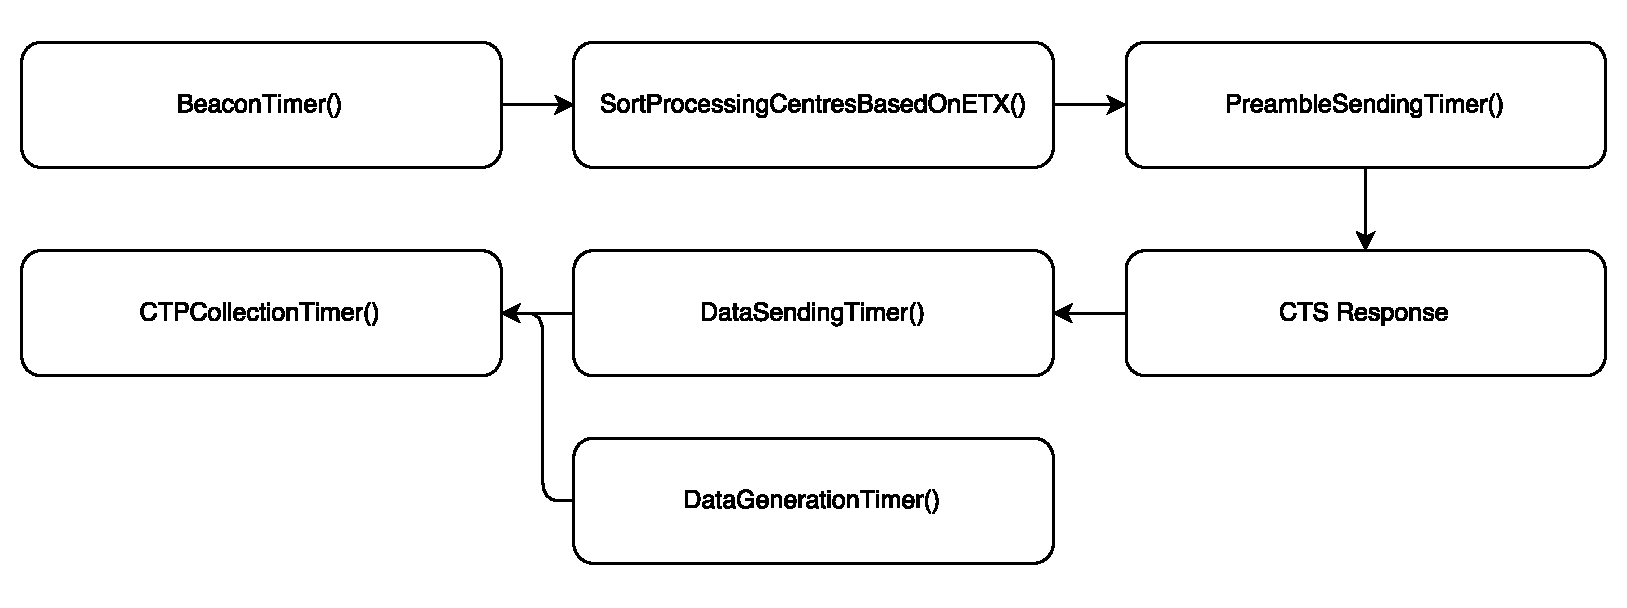
\includegraphics[width=1.0\textwidth]{gfx/TimerWorkflowSummarised.pdf}
    \caption{Timer Work Flow Summarised}
    \label{fig:TimerWorkflowSummarised}
    \end{figure}
	
	In subsection \ref{subsec:TimersFlowchartDiagrams}, we will differentiate the timers for different types of \acp{SN}. And in the further subsections we will discuss these timer

	%************************************************
	\subsection{Timers Flowchart Diagrams}\label{subsec:TimersFlowchartDiagrams}
	%************************************************
	
	\begin{figure}
    \centering
    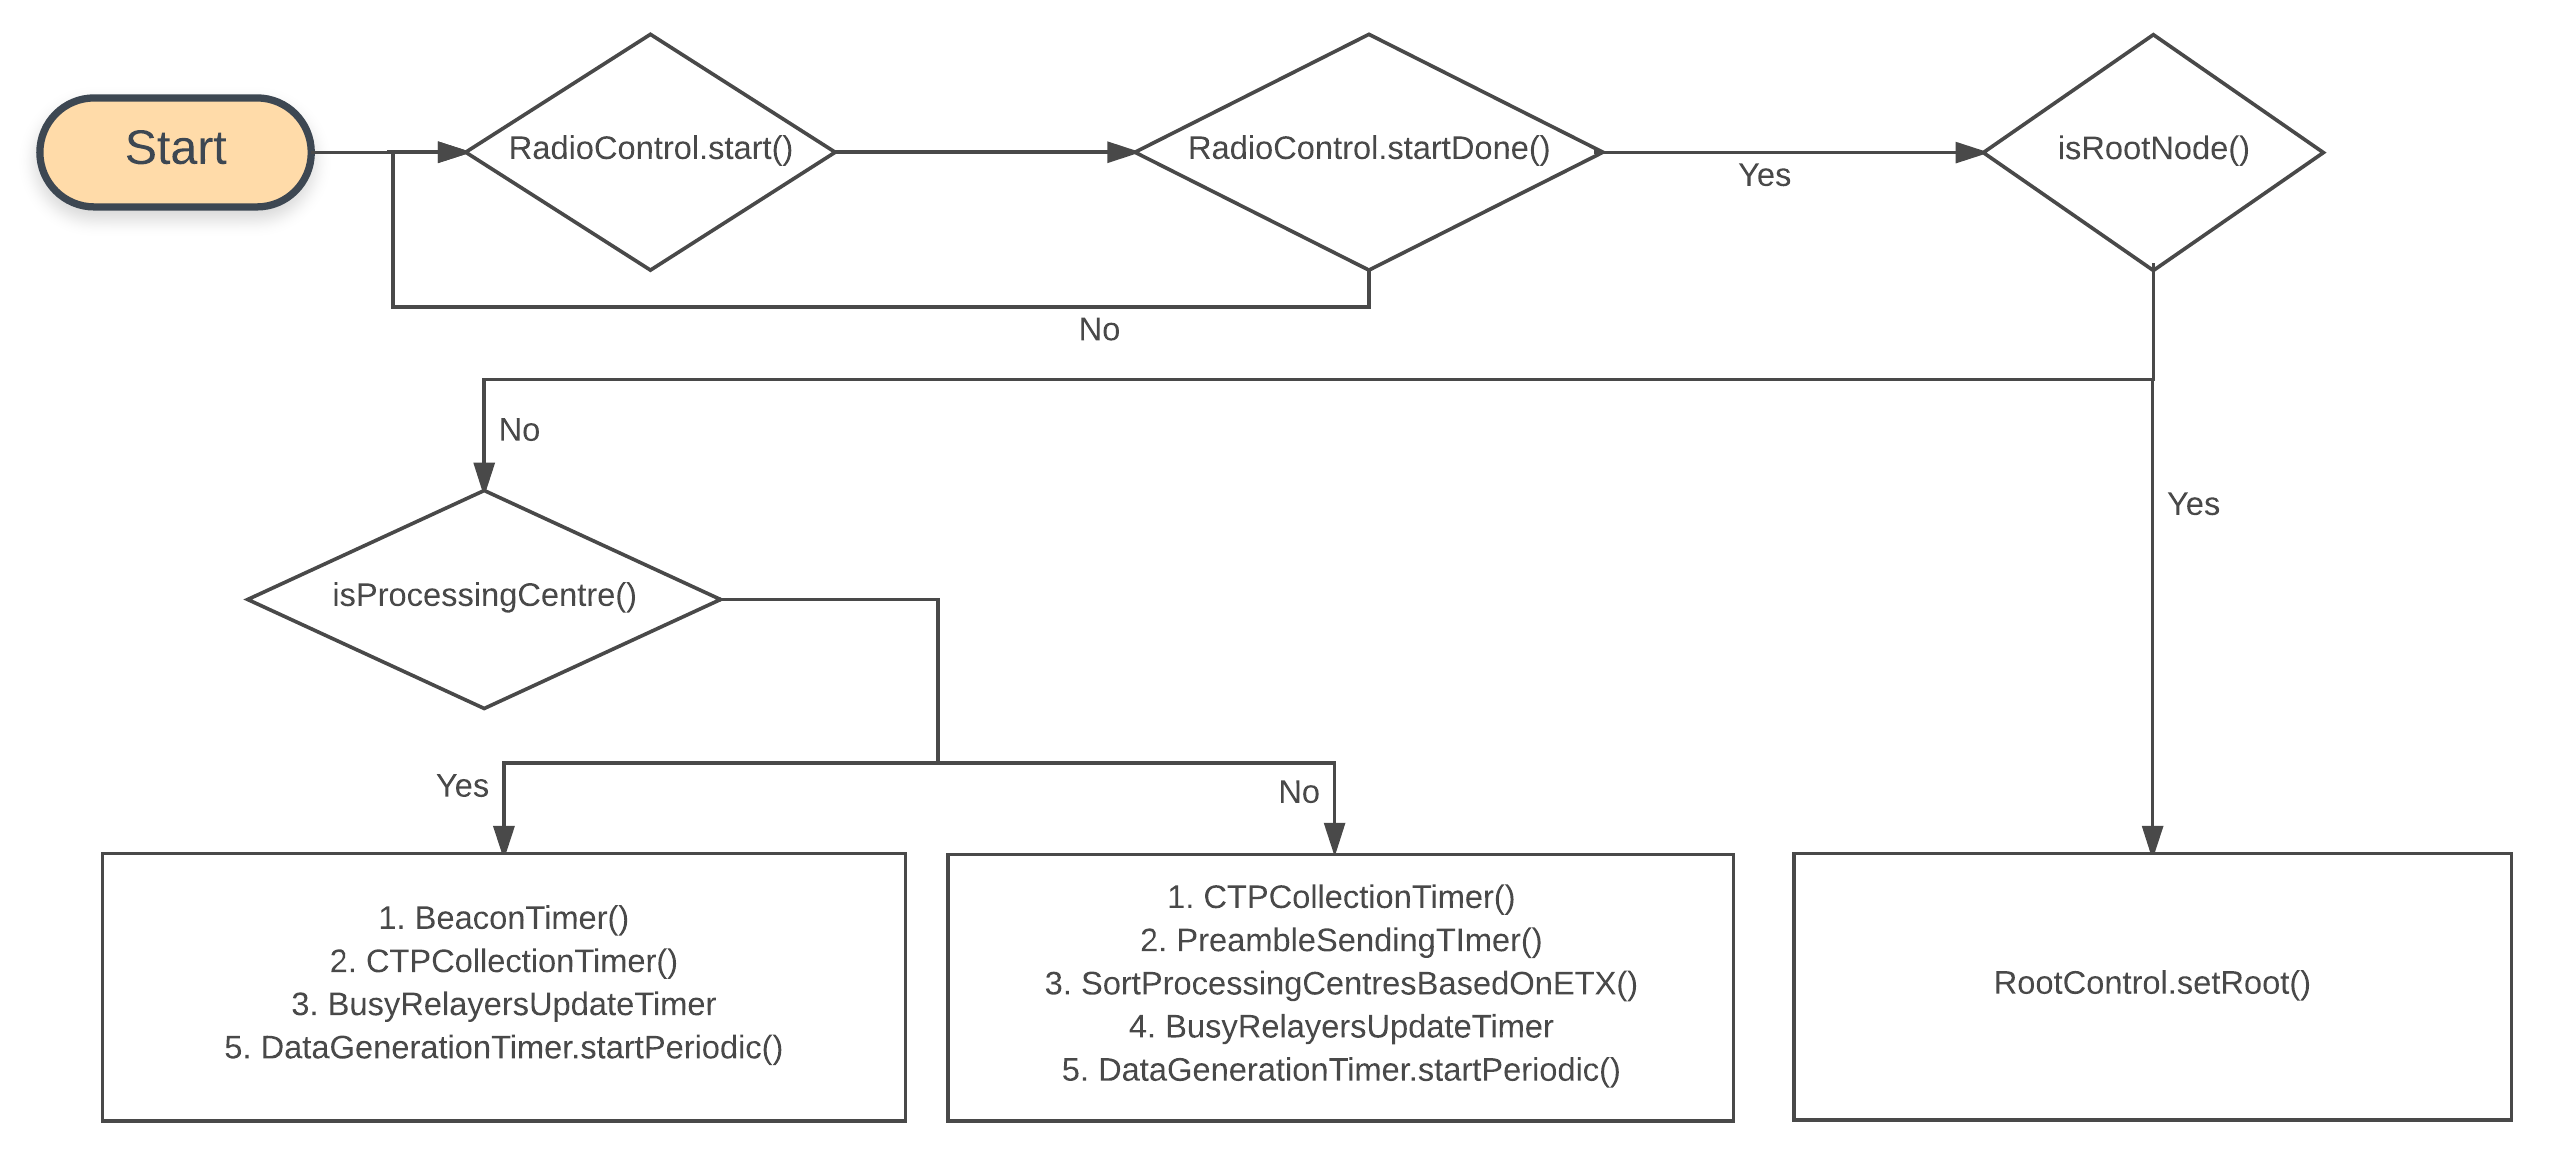
\includegraphics[width=1.0\textwidth]{gfx/Flow_diagram_start.png}
    \caption{Timer Interfaces in Heterogeneity}
    \label{fig:TimerInterfaces}
    \end{figure}

	
	In figure \ref{fig:TimerInterfaces}, we have illustrated a flow chart for the lifecycle of a \ac{SN} participating in heterogeneity design. Initially, every \ac{SN} turns it radio transceivers on and then, only when the RadioStart.startDone event signals without any errors, the \ac{SN} proceeds further to start certain timers. The selection of timers is based on two methods:
	
	\begin{enumerate}
	    \item isProcessingCentre: This method returns True, if the address of the current \ac{SN} (obtained by TOS\_NODE\_ID) matches a list of \acp{PC} defined as enum constants.
	    
	    \item isRootNode: This method returns True, if the address of the current \ac{SN} (obtained by TOS\_NODE\_ID) matches a list of \acp{BS} defined as enum constants.
	\end{enumerate}
	
	Based on the return values, appropriate timers are triggered. We will look at these timers in detail in coming subsections.
	    	
	%************************************************
	\subsection*{BeaconTimer}
	%************************************************
    
    It is a periodic timer fired by \ac{PC} at regular intervals. Figure \ref{fig:BeaconTimer} explains this concept in more detail. Firstly, each of the \acp{PC} checks sendBusyBeacon flag. If the flag is found not busy, a beacon, consisting of \ac{ETX} and \ac{PC}id, is broad-casted in one-hop neighborhood. On reception of these beacons, the \ac{SN} first update their local copy of processing centre struct array, which consists of \ac{PC} id, \ac{PC} \ac{ETX}, relayer id and relayer \ac{ETX} and then they forward it to their one hop neighbors. In the next subsection, we explain the PreambleSending Timer diagram which uses these updated local copy of \ac{PC} to send \ac{RTS} packets.

	\begin{figure}
    \centering
    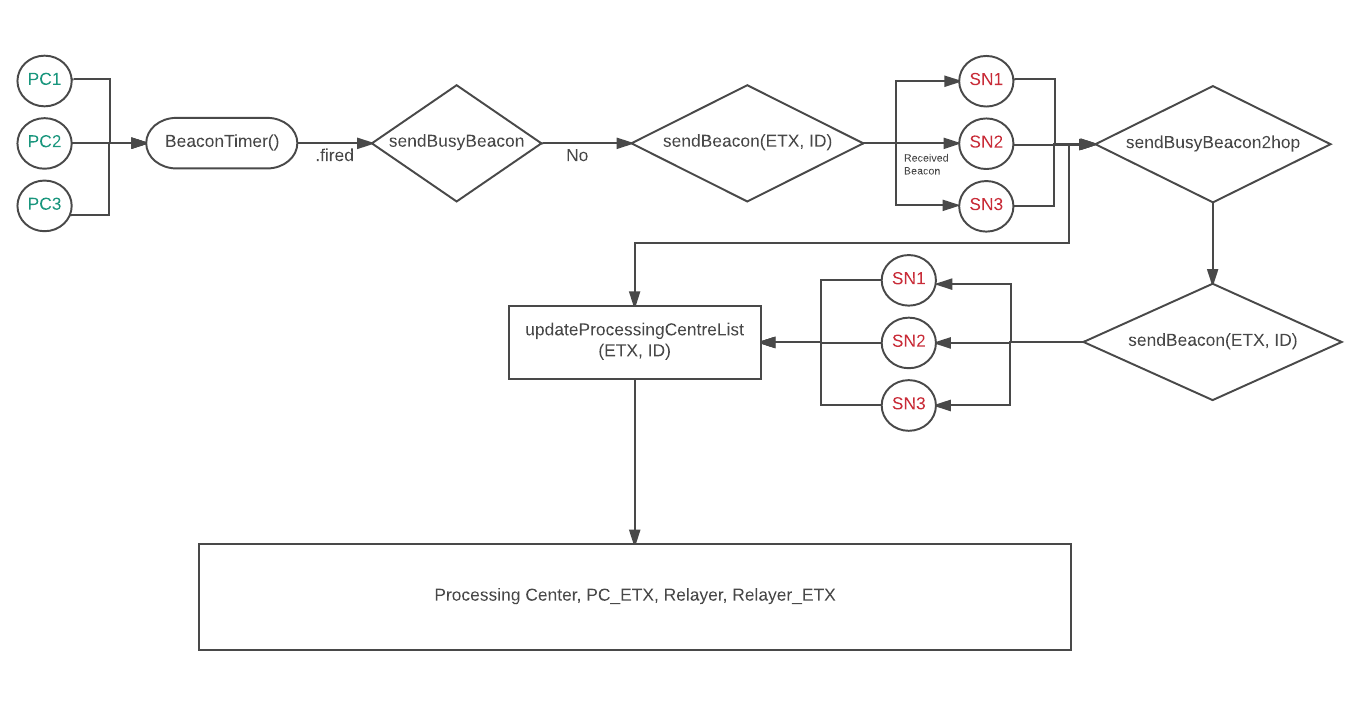
\includegraphics[width=1.0\textwidth]{gfx/BeaconTimer.png}
    \caption{Beacon Timer}
    \label{fig:BeaconTimer}
    \end{figure}
    
	%************************************************
	\subsection*{PreambleSendingTimer}
	%************************************************
	
	Each \ac{SN} maintains an updated list of \acp{PC} in two hop neighborhood and further sends a \ac{RTS} packet to request data processing by a \ac{PC}, based on the current state (occupied or free) of the \ac{SN}. We will explain this concept with the help of figure \ref{fig:PreambleTimer}. The model requires the sorted data from \textit{SortProcessingCentresBasedOnETX} timer. This timer periodically sorts the data in processing centre struct array based on lowest \ac{ETX} value and neighborhood distance. The PreambleSendingTimer then uses two arrays to decide whom to send \ac{RTS}: 1. sorted array of \acp{PC} and 2. busy \acp{PC} and relayers struct array (initially this list is empty, which means no \ac{PC} is busy initially). If a \ac{PC} is found by the method getProcessingCentreForTransmission using the above mentioned arrays, a \ac{RTS} packet is sent by setting transmitter address, receiver address, relayer address and duration of transfer desired as the packet contents. The recipient verifies if it is a relayer by extracting the relayer address from the packet contents (for a relayed transmission the packet content will have non-zero relayer address). In relayed transmission case, the packet is further forwarded to destination \ac{PC}. On reception of \ac{RTS} request by the \ac{PC}, it queues the request in CTSQueue and sends the \ac{CTS} response to the first \ac{RTS} sender. The sending response is broad-casted so that spectator \acp{SN} update their busy \acp{PC} and realyers struct array. This prevents other senders from not selecting an already occupied \ac{PC}. After getting the \ac{CTS} response, DataSendingTimer is fired which initiates the data transmission phase. The flowchart for DataSendingTimer is explained in next subsection.
	
	\begin{figure}
    \centering
    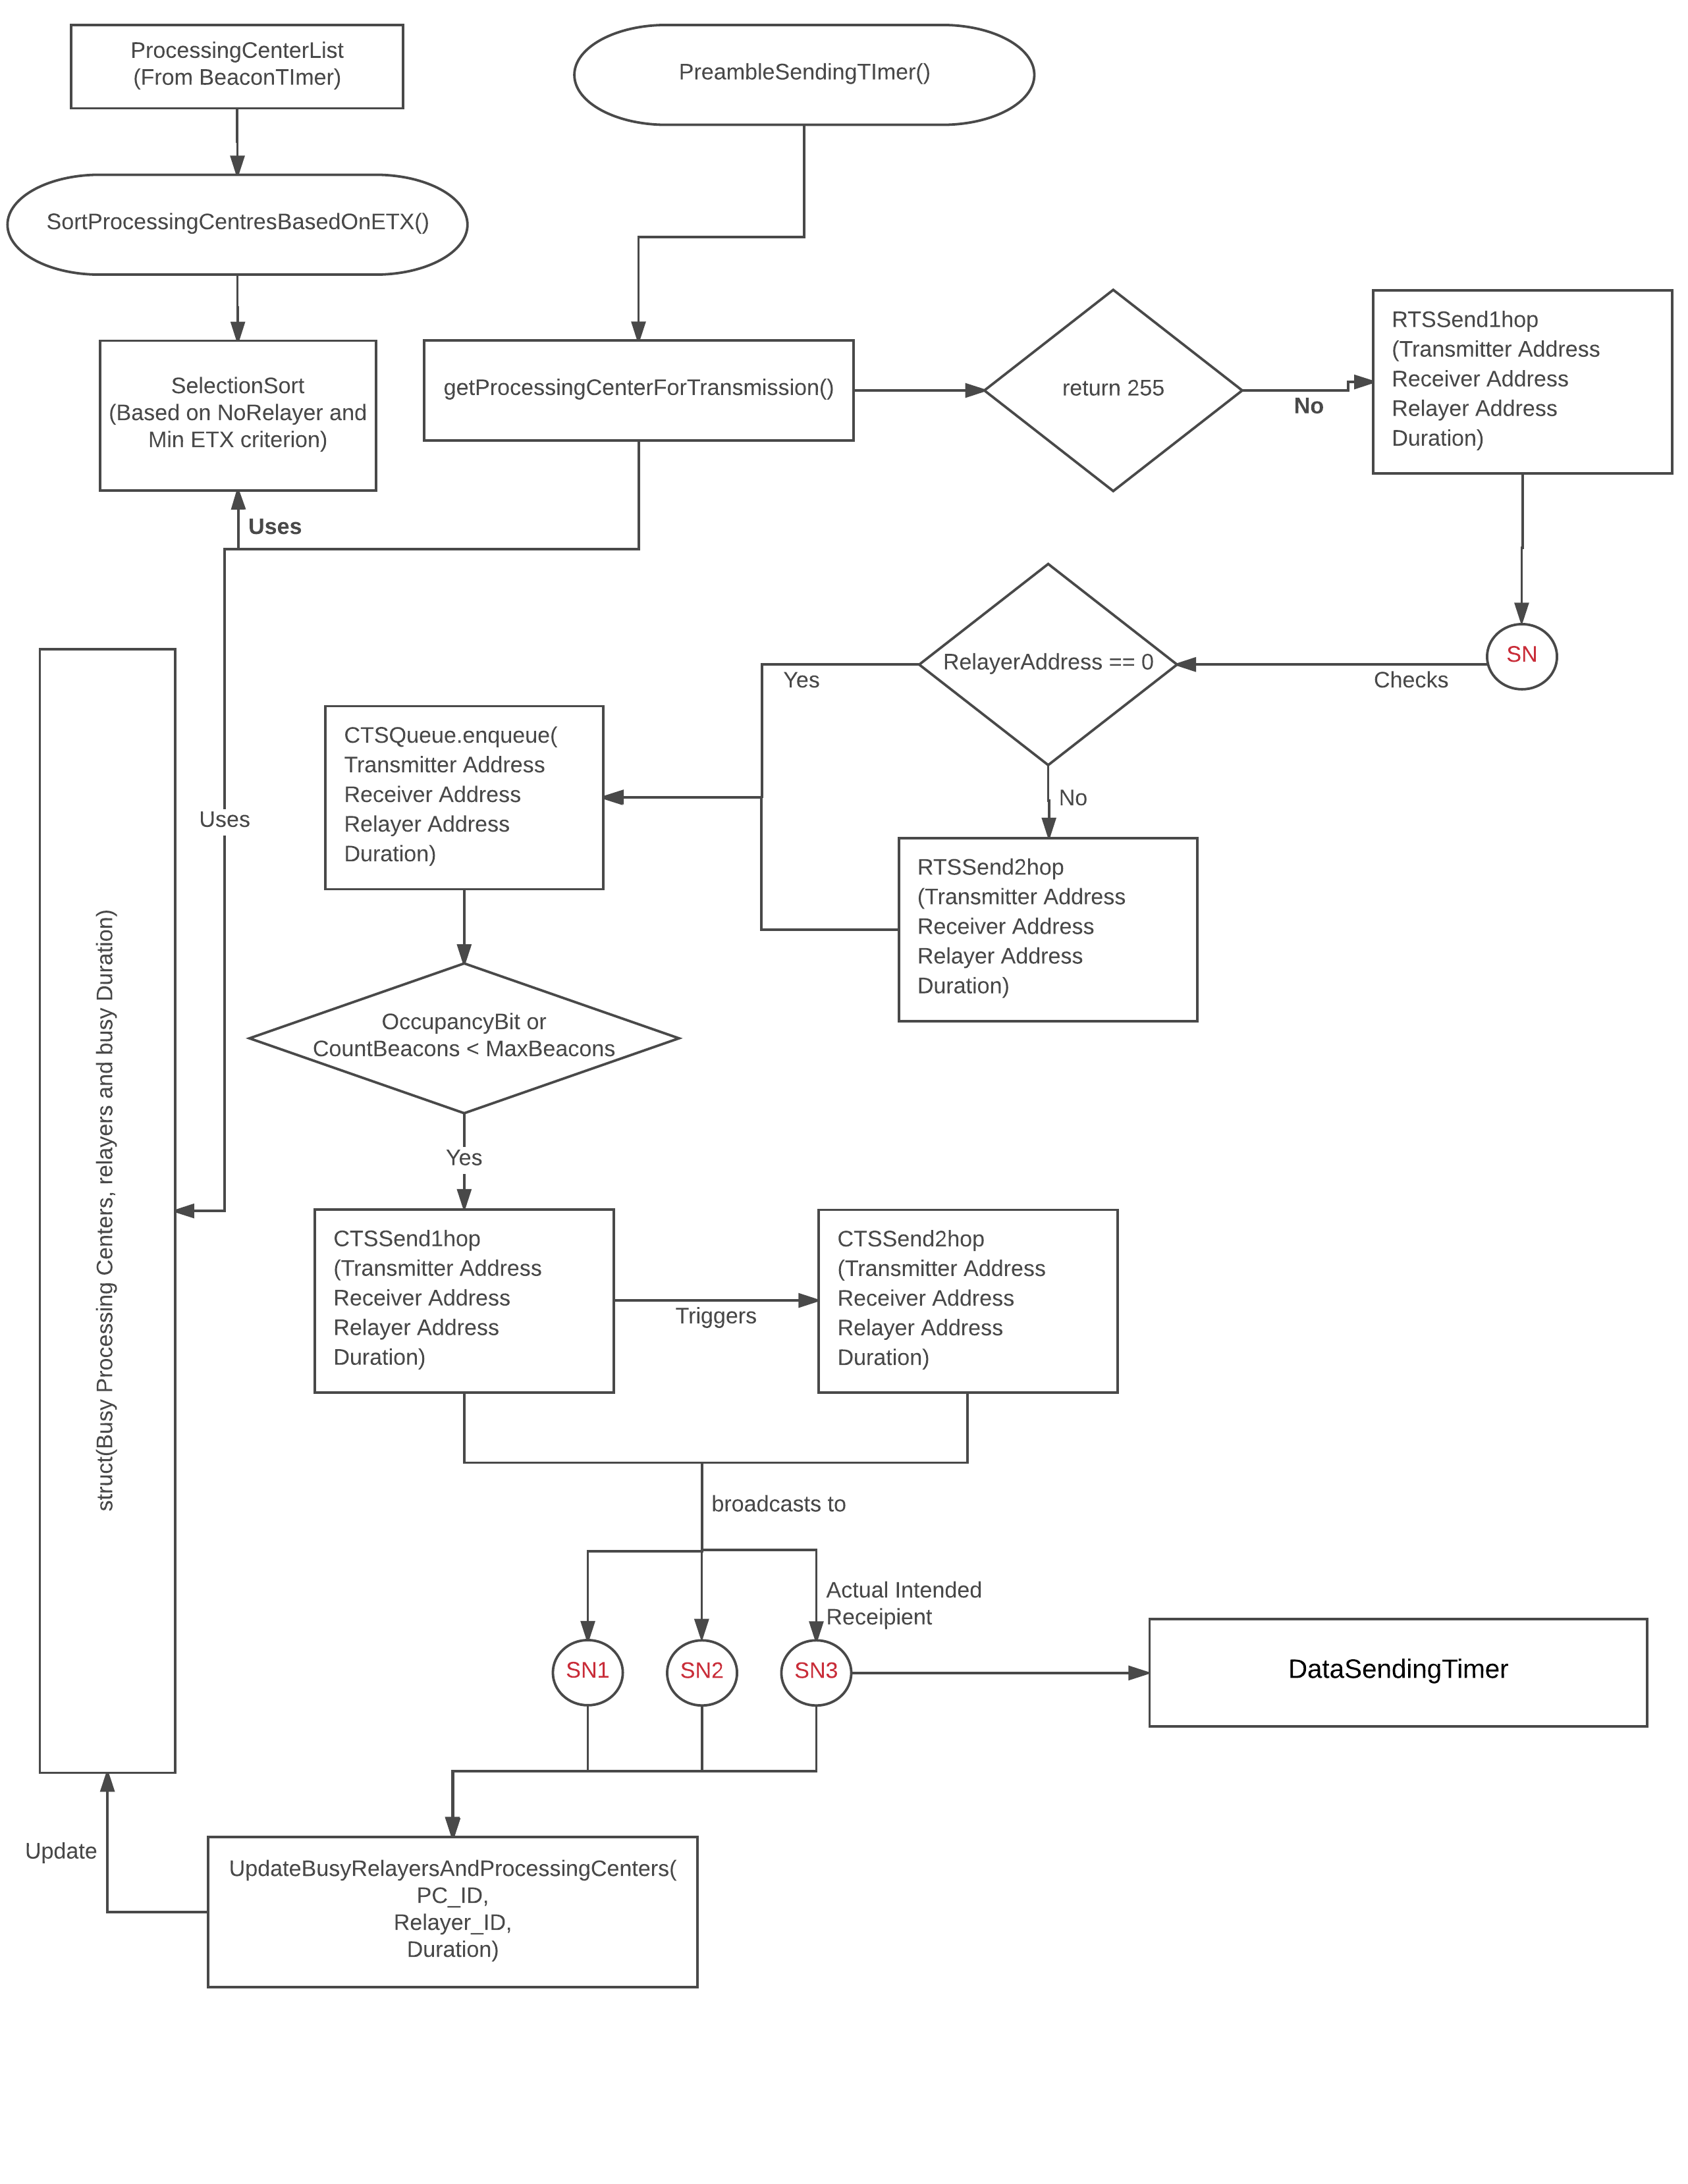
\includegraphics[width=1.0\textwidth]{gfx/PreambleSendingTimer.png}
    \caption{Beacon Timer}
    \label{fig:PreambleTimer}
    \end{figure}
    
	%************************************************
	\subsection*{DataSendingTimer}
	%************************************************
	
	DataSendingTimer is triggered only after \ac{RTS} response has been made by \ac{PC}. Figure \ref{fig:DataSendingTimer} elaborates the data sending concept of heterogeneity model in detail. Once data sending timer is fired, the intended sender verifies whether the time allotted to it is still remaining. If this condition holds, data is sent to the \ac{PC} or one hop relayer depending on whether it is one hop transmission or two hop transmission respectively. The AMSend.send signals send.sendDone event after successful or unsuccessful data transmission. We utilise this signalling event to again call data sending timer for sending the next packet. 
	
	\begin{figure}
    \centering
    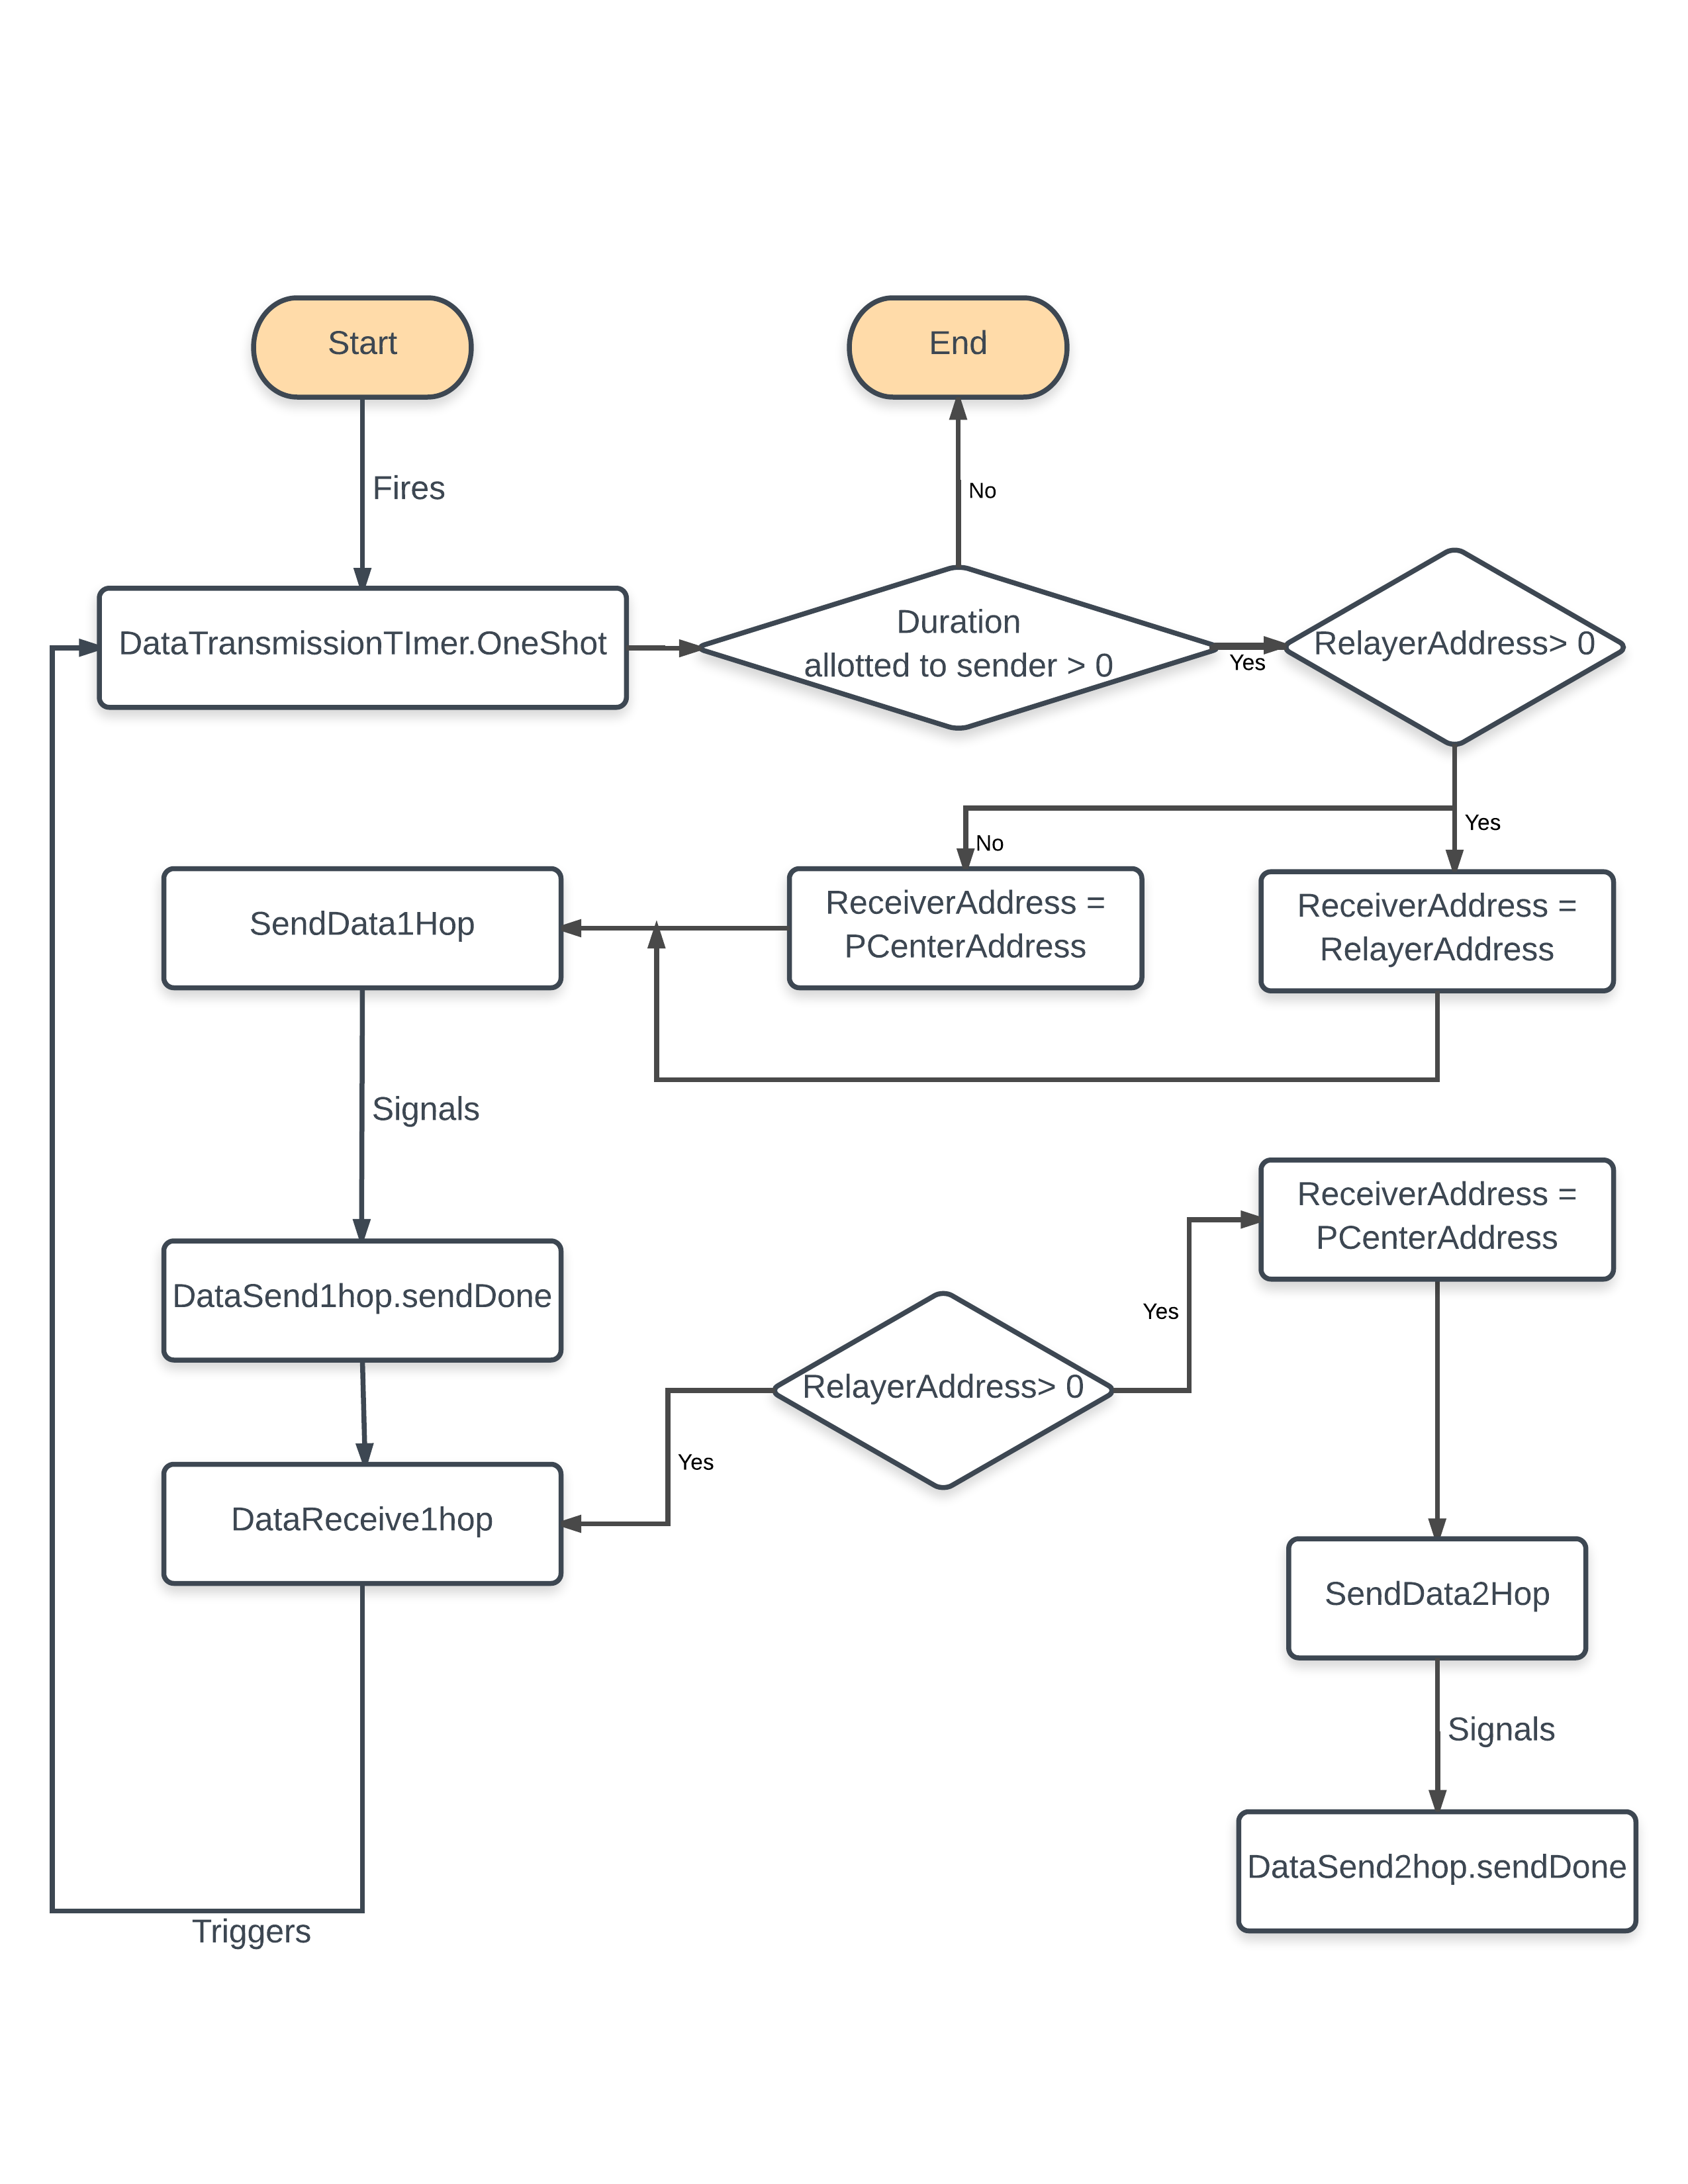
\includegraphics[width=1.0\textwidth]{gfx/DataSendingTimer.png}
    \caption{Data Sending Timer}
    \label{fig:DataSendingTimer}
    \end{figure}
    
        
	%************************************************
	\subsection*{CTPSendingTimer}
	%************************************************
	
	Data received by \ac{PC} is computed and added to CTPCollectionDataQueue. CTPTimer fires periodically and collects this data to route it via \ac{CTP} to \ac{BS}. If there are no elements in this queue, the timer uses DataGenerationQueue to route data via \ac{CTP}. DataGenerationQueue contains data acquired periodically by the \ac{SN}. For demonstrating heterogeneity, we have generated random numbers by periodically firing DataGenerationTimer. 
	This concept is shown in flowchart \ref{fig:CTPSendingTimer}.
    
    \begin{figure}
    \centering
    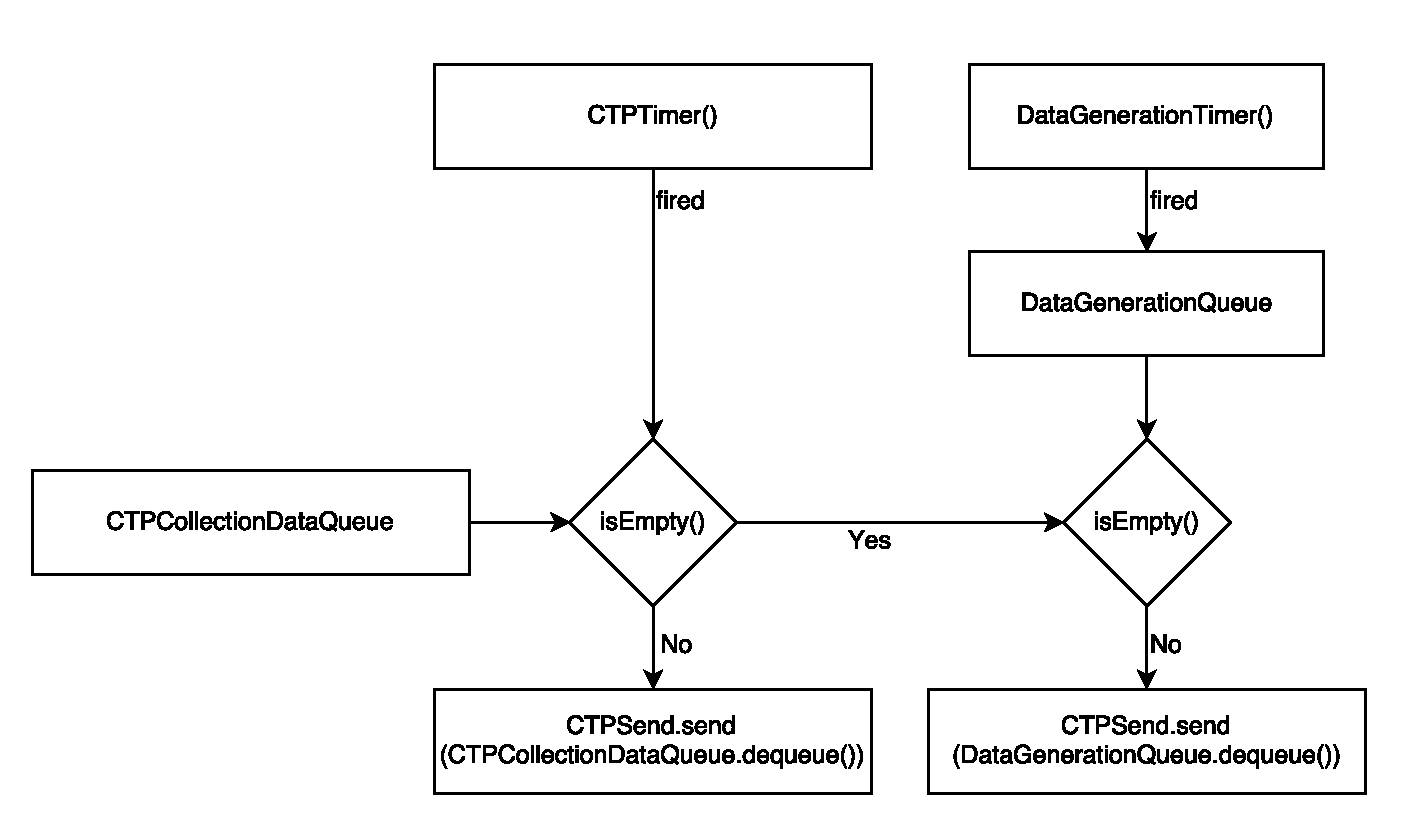
\includegraphics[width=1.0\textwidth]{gfx/CTPSendingTimer.pdf}
    \caption{\ac{CTP} Sending Timer}
    \label{fig:CTPSendingTimer}
    \end{figure}

% How the whole model looks as a process. What is the input and what is the output
% How the entire system looks like from a black box point of view.
% How do we regulate the concepts to make the ideas work?
% Keeping information upto date on timely basis
% Transition from the concept of timers to real time monitoring and checking of data transmission
    

